\documentclass{tufte-handout}

\usepackage{ntheorem}
\usepackage{graphicx}
\usepackage{amsmath}
\usepackage{amssymb}
\usepackage{hyperref}
\usepackage{epigraph}
\usepackage{booktabs}
\theoremstyle{break}
% \usepackage[
% bibencoding=utf8,% .bib file encoding
% maxbibnames=3, % otherwise et al
% minbibnames=1, % otherwise et al
% backend=biber,%
% sortlocale=en_US,%
% style=apa,% or authoryear
% % apabackref=false, % backreferences
% natbib=true,% for citet/citep, but this is for backward compatibility
% uniquename=false,%
% url=true,%
% sortcites=false,
% doi=true,%
% eprint=true%
% ]{biblatex}
% \addbibresource{lecture_note_bib.bib}

\hypersetup{
  colorlinks,
  urlcolor = blue,
  pdfauthor={Paul Goldsmith-Pinkham}
  pdfkeywords={econometrics}
  pdftitle={Lecture Notes for Applied Empirical Methods}
  pdfpagemode=UseNone
}
\newtheorem{ruleN}{Rule}
\newtheorem{thmN}{Theorem}
\newtheorem{assN}{Assumption}
\newtheorem{defN}{Definition}
\newtheorem{exmp}{Example}
\newtheorem{cmt}{Comment}
\newtheorem{proof}{Proof}

\newcommand{\continuation}{??}
\newtheorem*{excont}{Example \continuation}
\newenvironment{continueexample}[1]
 {\renewcommand{\continuation}{\ref{#1}}\excont[continued]}
 {\endexcont}
\newcommand{\bY}{\mathbf{Y}}
\newcommand{\bX}{\mathbf{X}}
\newcommand{\bD}{\mathbf{D}}
\newcommand{\E}{\mathbb{E}}

\newcommand\independent{\protect\mathpalette{\protect\independenT}{\perp}}
\def\independenT#1#2{\mathrel{\rlap{$#1#2$}\mkern2mu{#1#2}}}
\DeclareMathOperator{\Supp}{Supp}

\usepackage{cleveref}
\crefname{appsec}{appendix}{appendices}
\crefname{appsubsec}{appendix}{appendices}
\crefname{assumption}{assumption}{assumptions}
\crefname{equation}{equation}{equations}
\crefname{exmp}{example}{examples}
\crefname{assN}{assumption}{assumptions}
\crefname{cmt}{comment}{comments}
\crefname{defN}{definition}{definitions}

\usepackage[nolist]{acronym}
\begin{acronym}
  \acro{CI}{confidence interval}%
  \acro{OLS}{ordinary least squares}%
  \acro{CLT}{central limit theorem}%
  \acro{IV}{instrumental variables}%
  \acro{ATE}{average treatment effect}%
  \acro{RCT}{randomized control trial}%
  \acro{SUTVA}{stable unit treatment value assignment}
  \acro{VAM}{value-added model}%
  \acro{LAN}{locally asymptotically normal}%
  \acro{DiD}{difference-in-differences}%
  \acro{OVB}{omitted variables bias}
  \acro{FWL}{Frisch-Waugh-Lovell}
  \acro{DAG}{directed acyclic graph}
  \acro{PO}{potential outcomes}
\end{acronym}

\def\inprobHIGH{\,{\buildrel p \over \rightarrow}\,} 
\def\inprob{\,{\inprobHIGH}\,} 
\def\indistHIGH{\,{\buildrel d \over \rightarrow}\,} 
\def\indist{\,{\indistHIGH}\,}

\usepackage[many]{tcolorbox} 
\definecolor{main}{HTML}{5989cf}    % setting main color to be used
\definecolor{sub}{HTML}{cde4ff}     % setting sub color to be used
\definecolor{sub2}{HTML}{fde9ce}     % setting sub color to be used

\tcbset{
    sharp corners,
    colback = white,
    before skip = 0.2cm,    % add extra space before the box
    after skip = 0.5cm      % add extra space after the box
}                           % setting global options for tcolorbox

\newtcolorbox{boxD}{
    colback = sub, 
    colframe = main, 
    boxrule = 0pt, 
    toprule = 3pt, % top rule weight
    bottomrule = 3pt % bottom rule weight
}


\newtcolorbox{boxF}{
    colback = sub2,
    enhanced,
    boxrule = 1.5pt, 
    colframe = white, % making the base for dash line
    borderline = {1.5pt}{0pt}{main, dashed} % add "dashed" for dashed line
}

\usepackage{colortbl}


\usepackage{tikz}
\usepackage{verbatim}
\usetikzlibrary{positioning}
\usetikzlibrary{snakes}
\usetikzlibrary{calc}
\usetikzlibrary{arrows}
\usetikzlibrary{decorations.markings}
\usetikzlibrary{shapes.misc}
\usetikzlibrary{matrix,shapes,arrows,fit,tikzmark}

\title{Lecture 3 - Propensity Scores}
\author{Paul Goldsmith-Pinkham}
\date{\today}


\begin{document}

\maketitle
For today, propensity scores. The end goal: 
    \begin{itemize}
    \item Have a framework for discussing subpopulations
      being treated
    \item A way to link to an underlying economic model
    \end{itemize}
This will provide structure for us later
 
\section{Propensity score weighting}

Begin by recalling our definition of conditional strong ignorability:
\begin{defN}
    \label{def:strong_ignorability}
    We say that $D_{i}$ is strongly ignorable conditional on a vector $\bX_{i}$ if
    \begin{enumerate}
  \item     $Y_{i}(0), Y_{i}(1) \perp D_{i} | \bX_{i}$
  \item $\exists \varepsilon > 0$ such that $\varepsilon < Pr(D_{i} = 1 | \bX_{i}) < 1-\varepsilon$.
    \end{enumerate}
  \end{defN}
The important feature that we will engage with today is how conditional strong ignorability can depend on a potential complex and high-dimensional vector $\bX$. When $\bX$ is complex, it can be challenging to consider how to implement the ATE estimator as we constructed in our proof. Namely, estimating the CATE $\tau(x)$ for all $x$ may be challenging.

What we will explore today is how the \emph{propensity score} can be used to elide this problem. Let $\pi(\bX_{i}) \equiv E(D_{i} | \bX_{i}) = Pr(D_{i} | \bX_{i})$ be the probability of treatment conditional on $\bX$. The propensity score is a scalar summary of the high-dimensional $\bX$.\footnote{A student of linear regression might notice that the propensity score is analagous to the auxiliary regression of a regression setup of $Y_{i}$ on $\bX_{i}$ and $D_{i}$. In essence, the propensity score captures the bias in the coefficient on $D_{i}$ that would occur from omitting $\bX$ from the main regression.}

A key result from \citet{rosenbaum1983central}\footnote{Aptly named ``The Central Role of the Propensity Score in Observational Studies for Causal Effects.''} is that if  
$$Y_{i}(0), Y_{i}(1) \perp D_{i} | \bX_{i}$$ 
holds, then so does  $Y_{i}(0), Y_{i}(1) \perp D_{i} | \pi(\bX)$. The propensity score here acts as the coarsest possible ``balancing score'' such that the distribution of $\bX$ is the same for both the treated and control groups. Why is this useful? It solves a high-dimensional problem -- instead of exactly matching on many different values in $\bX$, we only have to worry about a single scalar $\pi(\bX)$.

Conditioning on a single propensity score is a slightly weaker condition than conditioning on the full vector $\bX$. However, it opens up new questions and estimation issues. 

\begin{enumerate}
    \item  First, how do we estimate the propensity score? When $\bX$ is discrete, we can estimate $\pi(\bX)$ non-parametrically by calculating $E(D_{i} | \bX_{i} = x)$ for every $x$ value, but that may ask quite a bit of the data. An alternative approach is to assume a model for $\pi(\bX)$, such as a logistic regression model. This is a parametric approach, but it can be more efficient if the model is correctly specified. A third approach is to use a parametric model but to include flexible terms for $\bX$ to allow for non-linearities. This is a semi-parametric approach, and it can be more flexible than the fully parametric approach.
    \item Second, once we have an estimated $\pi(\bX)$, how do we use it to construct the ATE or other estimands? If we directly treat it as a covariate, it becomes a bit challenging, as we discover in \Cref{example:aronow_matching}. Instead, we will use another beautiful result from \citet{rosenbaum1983central} that shows how we can use the Horvitz-Thompson estimator to construct the ATE using the propensity score.
\end{enumerate}

\subsection{Horvitz-Thompson Estimator}
Recall our estimator for the average treatment effect from last lecture, the \underline{Horvitz-Thompson estimator}:\footnote{This is sometimes referred to as the inverse propensity score (or weighting) (IPW) estimator. But if you want to seem fancy you can call it the HOrvitz-Thompson estimator. Impress your statistics colleagues!}
\begin{defN}
    We observe a sample of $(Y_{i}, X_{i}, D_{i})$ triples for $n$ observations. Let $\pi(\bX_{i}) = Pr(D_{i} = 1 | \bX_{i})$ be the \textbf{propensity score} and define the \textbf{Horvitz-Thompson estimator} for the average treatment effect as:
    \begin{align*}
        \hat{\tau}_{HT} = n^{-1} \sum_{i=1}^n \frac{D_i Y_i}{\pi_i(X_{i})} - n^{-1} \sum_{i=1}^n \frac{(1-D_i) Y_i}{1-\pi_i(X_{i})}
    \end{align*}
\end{defN}

This estimator is the direct empirical analog to the following population result:
\begin{equation*}
  E(\tau_{i}) = E\left(\underbrace{\frac{Y_{i}D_{i}}{\pi(\mathbf{X})}}_{E(Y_{i}(1))} - \underbrace{\frac{Y_{i}(1-D_{i})}{1-\pi(\mathbf{X})}}_{E(Y_{i}(0))}\right)
\end{equation*}
This problem takes advantage of the estimand of interest, rather than tryign to address the problem literaly by estimating every CATE and weighting up accordingly.\footnote{Convince yourself that under discrete and few $X$, this collapses to what we would logically do anyway. With many $X$, you typically may be willing to make modeling assumptions on $\pi$ for efficiency reasons.}


\begin{boxD}
    \begin{exmp}[Propensity score matching]
        \label{example:aronow_matching}
        Consider the following example from \citet{aronow2019foundations}, with 6 observations and two variables $X_{i1}$ and $X_{i2}$:

        \centering
\begin{tabular}{ccccccc}
    \toprule
    $i$ & $Y_{i}(0)$ & $Y_{i}(1)$ & $D_{i}$ & $X_{i1}$ & $X_{i2}$ & $\pi(\mathbf{X}_{i})$\\
    \midrule
    1 & - & 2 & 1 & 1 & 7 & 0.33\\
    2 & 5 & - & 0 & 0 & 7 & 0.14\\    
    3 & - & 3 & 1 & 10 & 3 & 0.73\\
    4 & - & 10 & 1 & 3 & 1 & 0.35\\
    5 & - & 2 & 1 & 5 & 2 & 0.78\\
    6 & 0 & - & 0 & 7 & 0 & 0.70\\
    \bottomrule
  \end{tabular}

  \raggedright
  \hspace{10pt}Ideally, we would match observations based on the exact propensity score, but as we can already see in this example, no two observations have the same $\pi(\bX)$. Instead, we have to approximate matches. This will create bias unless we assume that the distance will shrink as our number of observations grows. 

  \hspace{10pt}It becomes a question of exactly how to construct the matches, and how many matches to choose. Do you pick just the closest neighbor? All neighbors within a fixed distance? This is a complicated problem that can affect inference and discussed in \citet{abadie2008failure}. As an example, consider what happens if we impute based on the closest neighbor for each observation: 

  \centering
  \begin{tabular}{ccccccc}
    $i$ & $Y_{i}(0)$ & $Y_{i}(1)$ & $D_{i}$ & $X_{i1}$ & $X_{i2}$ & $\pi(\mathbf{X}_{i})$\\
    \midrule
    1 & \textcolor{red}{5} & 2 & 1 & 1 & 7 & 0.33\\
    2 & 5 & \textcolor{red}{2} & 0 & 0 & 7 & 0.14\\    
    3 & \textcolor{red}{0} & 3 & 1 & 10 & 3 & 0.73\\
    4 & \textcolor{red}{5} & 10 & 1 & 3 & 1 & 0.35\\
    5 & \textcolor{red}{0} & 2 & 1 & 5 & 2 & 0.78\\
    6 & 0 & \textcolor{red}{3} & 0 & 7 & 0 & 0.70\\        
  \end{tabular}

  \raggedright
  \hspace{10pt}In this case, several units are used more than once as matches. Moreover, there are very close ``ties'': we picked unit $i=1$ for unit $2$, but unit $4$ was very close as well. Why not pick that one, especially with $\pi(\bX)$ is noisy? This is a difficult problem to solve, and it is not clear that there is a single best answer.
    \end{exmp}
\end{boxD}

The Horvitz-Thompson estimator works well but in smalll samples can be high variance if $\pi(\bX)$ is close to zero or one. This can be improved through the use of \emph{stabilized weights}:
\begin{equation*}
    \hat{\tau}_{SIPW} = \frac{\frac{1}{n}\sum_{i}\frac{Y_{i}D_{i}}{\hat{\pi}(\mathbf{X}_{i})}}{\frac{1}{n}\sum_{i}\frac{D_{i}}{\hat{\pi}(\mathbf{X}_{i})}} - \frac{\frac{1}{n}\sum_{i}\frac{Y_{i}(1-D_{i})}{1-\hat{\pi}(\mathbf{X})}}{\frac{1}{n}\sum_{i}\frac{(1-D_{i})}{1-\hat{\pi}(\mathbf{X})}}
  \end{equation*}

This estimator benefits by adjusting for unusually high or low values of $\pi(\mathbf{X})$ by constructing weights $w_{i} = \frac{\frac{D_{i}}{\hat{\pi}(\mathbf{X}_{i})}}{\frac{1}{n}\sum_{i}\frac{D_{i}}{\hat{\pi}(\mathbf{X}_{i})}} $ for the treated group.\footnote{In the limit, recall that $\frac{1}{n}\sum_{i}\frac{D_{i}}{\hat{\pi}(\mathbf{X}_{i})}$ should converge to 1 (since $E(\pi^{-1}(\bX_{i})D_{i}) = 1$), and hence the SIPW converges to the IPW.} Similar to the IPW, this is also an unbiased estimator of the ATE.

\begin{boxF}
\begin{cmt}[True versus estimated propensity scores]
 When an intervention is truly randomly assigned, the propensity score itself is known. However, in most non-experimental settings, the p-score is unknown and must be estimated. As we discussed above, we need to estimate $\pi(X)$ and it can be done in parametric, semi-parametric, or non-parametric fashion, depending on your assumptions about $\bX$. 

 \hspace{10pt}It is useful to note that the model used to estimate the propensity score matters. For example, the linear probability model, which is commonly used for many binary outcomes, may predict probabilities for the propensity score that are outside the range of $[0,1]$, thereby generating improper IPW estimates. The LPM will work if the model is fully saturated and non-parametric (e.g. a set of fully interacted dummies), but this is not always the case. 


 \hspace{10pt}Another important result in this literature is that \emph{even if you know the true function $\pi(\mathbf{X})$}, you are better off using the estimated function than the true $\pi(\bX)$ \citep{hirano2003efficient}. The intuition for this result is that the deviations from the ``true'' propensity score ($\hat{\pi}(\mathbf{X}) - \pi(\mathbf{X})$) are informative for the estimation of the treatment effects (a la extra moment restrictions in GMM)

\end{cmt}
\end{boxF}

\subsection{Contrasting linear regression with propensity scores}


Say we have strong ignorability conditional on $\bX$ and we run the following regression:
    \begin{equation}
      \label{eq:regression_imputation}
      Y_{i} = \gamma_{0} + D_{i}\beta + X_{i1}\gamma_{1} + X_{i2}\gamma_{2} + u_{i}.
    \end{equation}
How should we contrast this to the propensity score methods we used above? 

We can revisit the \citet{aronow2019foundations} example from \Cref{example:aronow_matching}, but instead of imputing for the missing counterfactual using matching, we impute using regression. 
 \begin{table*}
  \makebox[\textwidth]{%
  \begin{tabular}{ccccccc}
    $i$ & $Y_{i}(0)$ & $Y_{i}(1)$ & $D_{i}$ & $X_{i1}$ & $X_{i2}$ & $\pi(\mathbf{X}_{i})$\\
    \midrule
    1 & $\hat{\gamma}_{0} + \hat{\gamma}_{1} \cdot X_{i1} + \hat{\gamma}_{2} \cdot X_{i2}$  & 2 & 1 & 1 & 7 & 0.33\\
    2 & 5 & $\hat{\gamma}_{0} + \hat{\beta} + \hat{\gamma}_{1} \cdot X_{i1} + \hat{\gamma}_{2} \cdot X_{i2}$ & 0 & 0 & 7 & 0.14\\    
    3 & $\hat{\gamma}_{0} + \hat{\gamma}_{1} \cdot X_{i1} + \hat{\gamma}_{2} \cdot X_{i2}$ & 3 & 1 & 10 & 3 & 0.73\\
    4 & $\hat{\gamma}_{0}  + \hat{\gamma}_{1} \cdot X_{i1} + \hat{\gamma}_{2} \cdot X_{i2}$ & 10 & 1 & 3 & 1 & 0.35\\
    5 & $\hat{\gamma}_{0} + \hat{\gamma}_{1} \cdot X_{i1} + \hat{\gamma}_{2} \cdot X_{i2}$ & 2 & 1 & 5 & 2 & 0.78\\
    6 & 0 & $\hat{\gamma}_{0} + \hat{\beta}  + \hat{\gamma}_{1} \cdot X_{i1} + \hat{\gamma}_{2} \cdot X_{i2}$ & 0 & 7 & 0 & 0.70    
  \end{tabular}
  }
  \caption{Regression imputation in \citet{aronow2019foundations} example}
\end{table*}

This tells us, roughly speaking, what this regression approach will assume for the missing counterfactuals. Notably, this approach will do well when the conditional expectation function for the outcome (e.g. $E(Y_{i}(0)$)) is approximately linear in $\bX$ and $D_{i}$ -- e.g. you are roughly correctly specified. Importantly,  the approximation should not extrapolate too much across the support of $\mathbf{X}_{i}$.\footnote{To concretely give an example of how this could be an issue: note that unit $3$ is treated and is far out on the support of $\bX_{i}$ (10,3). Imputing values for that unit's control requires extrapolating quite far out on the support of $\bX_{i}$, which may be problematic unless the conditional mean is exactly correctly specified.} 

This is just another way to infer the missing data. However, a key issue is that if we just use OLS to estimate \Cref{eq:regression_imputation}, we will not necessarily recover the ATE with $\tau$. Recall that when $\bX$ is just a constant, then $tau$ is the ATE. Once we condition on covaraites, however, the estimand recovered by $\tau$ changes. We will revisit this in our linear regression lectures, but the key fact is that OLS will recover an estimand which is a different weighted average of the CATEs -- namely one that variance-weights the CATEs. 

First, it's useful to recall what we are assuming with strong ignorability. Recall that we are assuming that there is a function $E(D_{i} | \bX) \equiv \pi(\bX)$ that we can condition on such that there is no remaining correlation between $D_{i}$ and the potential outcomes. However, we do not know the function $\pi(\bX)$. If we are additionally willing to assume that $\pi(\bX) = X_{i1}\gamma_{1} + X_{i2}\gamma_{2}$, then by Frisch-Waugh-Lovell, we can show that $\tau$ will recover a weighted combination of the CATEs.\footnote{This discussion here follows \citet{angrist1998}, and is generally inspired by \citet{borusyak2024negative}.} Specifically, let $\tilde{D}_{i} = D_{i} - \pi(\bX_{i})$ and $\tau_{i} = Y_{i}(1) - Y_{i}(0)$. Then,
\begin{equation}
  \label{eq:ols_frac}
  \beta_{OLS} = \frac{E(\tilde{D}_{i}D_{i}\tau_{i})}{E(\tilde{D}_{i}^{2})}.
\end{equation}
As a result, the OLS coefficient will not necessarily estimate the ATE estimand. Instead, it will estimate a weighted average of the CATEs, where the weights are the variance of the treatment assignment conditional on $\bX$. We will revisit this during our linear regression lectures.

As a result, there are two key caveats with this approach: first, we need to be careful about how we specify the regression function with our $\bX$ variables. Especially if there is significant extrapolation across the support of $\bX$.\footnote{Note that in cases where we have two sets of fixed effects (e.g. age and location), we often just include the marginal fixed effects (e.g. age and location separately) and not the fully saturated specification(e.g. age $\times$ location). This is because the interaction fixed effects require too much of the data. However, there will consequentially be extrapolation that may be wrong.} Second, we need to be careful about how we interpret the coefficient on $D_{i}$ in the regression. It will not necessarily be the ATE, but instead a variance-weighted average of the CATEs. 



Consequentially, an important question for us as practitioners is which approach to use: IPW or regression? There are good reasons to like the IPW estimator for the ATE: \citet{hirano2003efficient} show that the IPW estimator is semiparametrically efficient when the propensity score is unknown.\footnote{However, the IPW estimator can be high variance when the propensity score is close to zero or one (this is known as weak overlap). This can create issues generally with estimating the ATE, and linear regression avoids this issue. See \citet{goldsmith2022contamination}.} But, linear regression is nice! It is straightforward to run, and easy to interpret. Moreover, it has been endorsed. From Angrist and Pischke (2009):
    \begin{quote}
      We believe regression should be the starting point for most empirical projects. This is not a theorem; undoubtedly, there are circumstances where propensity score matching provides more reliable estimates of average causal effects. The first reason we don't find ourselves on the propensity-score bandwagon is practical: there are many details to be filled in when implementing propensity-score matching - such as how to model the score and how to do inference - these details are not yet standardized. Different researchers might therefore reach very different conclusions, even when using the same data and covariates. Moreover, as we've seen with the Horvitz-Thompson estimands, there isn't very much theoretical daylight between regression and propensity-score weighting.
      \end{quote}



\begin{boxF}
  \begin{cmt}[Ex-Post Weights vs. Ex-Ante Weights]
    Note that in \Cref{eq:ols_frac},  
    $$\phi_{i}(\bX_{i}) = \tilde{D}_{i}D_{i}$$
     is a function of $\bX_{i}$ and can be negative. Then that means for some CATE ($E(\tau_{i} | \bX)$), there may be negative weights.  In some special cases, this will not be the case (e.g. $\pi(\bX)$ is correctly specified and/or $\bX$ is discrete and fully satuated).  These negative weights can be problematic because the weighted TE could then reflect an effect that does not exist in the underlying population at all.

    \hspace{10pt} However, as shown succinctly in \citet{borusyak2024negative}, the \emph{expected} ex ante weights in a design-based approach are guaranteed to be positive:  
    $$E(\phi_{i} | \bX_{i}, \beta_{i}) = Var(D_{i} | \bX_{i}, \beta_{i}) > 0.$$ 
    This implies, intuitively, that all units with the same $\bX_{i}$ will have the same weight prior to treatment. This is a key difference between the design-based approach and the model-based approach. This same statement cannot be done in a context where we model $E(Y_{i}(0))$ because we are not allowing the treatment to be randomly allocated across units (by)
  \end{cmt}
\end{boxF}

When we start worrying about the propensity score, life gets more complicated. It forces us to think about overlap of covariates and balance, namely how comparable the treated and untreated groups are. This became a key issue around the seminal NSW paper. 

\section{NSW and Propensity score matching}

There was a randomized intervention called the National Supported Work Demonstration (NSW), which was a temporary employment program to give work experience. A seminal paper by Lalonde \citep{lalonde1986evaluating} showed that a non-experimental analysis of this program  would have given biased estimates compared to experimental approach.\footnote{``This comparison shows that many of the econometric proce-
 dures do not replicate the experimentally determined results.''}


\citet{dehejia2002propensity,dehejia1999causal} reanalyze this data using propensity score methods, and argue that these results are more similar to the experimental results, relative to the non-experimental results proposed by \citet{lalonde1986evaluating}. Moreover, using propensity scores provides a form of diagnostics on how comparable the treated and control groups are.

It is worth digging in to the \citet{dehejia2002propensity} paper to understand how they use propensity scores. Crucial to their approach is they included the lagged outcomes as covariates in their approach. As a consequence, they  subsample the data to have two years of pre-treatment data. This is a key difference from the \citet{lalonde1986evaluating} approach, which used the full sample. \citet{smith2005does} assess this approach, and argue two points: first, the specification itself for the propensity score is quite sensitive to the choice of included variables.\footnote{In other words, deciding which variables to include in $\bX$ is important and can affect bias significantly. This echoes Leamer's critique on model specification in \citet{leamer1983let}.} Second, they argue that the \emph{subsampling} in \citet{dehejia2002propensity} predisposes to a group where the analysis is ``easy.'' Moreover, in this case difference-in-differences works best because it removes the time-invariant heterogeneity across units.

Dehijia's response in \citet{dehejia2005practical} is ``of course!'' -- the point of propensity score matching is to transparently highlight the assumptions in the data. More verbosely, he says:
\begin{quote}
  A judgment-free method for dealing with problems of sample selection bias is the Holy Grail of the evaluation literature, but this search reflects more the aspirations of researchers than any plausible reality. In practice, the best one can hope for is a method that works in an identifiable set of circumstances, and that is self-diagnostic in the sense that it raises a red flag if it is not functioning well. Propensity score methods are applicable when selection is based on variables that are observed. In the context of training programs, Dehejia and Wahba (1999, 2002), following on a suggestion from the training program literature (Ashenfelter, 1978; Ashenfelter and Card, 1985), suggest that two or more years of pre-treatment earnings are necessary. In terms of the self-diagnosis, the method and its associated sensitivity checks successfully identify the contexts in which it succeeds and those in which it does not succeed, at least for the NSW data. 
  
  \textbf{Propensity score matching does not provide a silver-bullet, black-box technique that can estimate the treatment effect under all circumstances}; neither the developers of the technique nor Dehejia and Wahba have claimed otherwise. However, with input and judgment from the researcher, it can be a useful and powerful tool. [Emphasis added]
\end{quote}

\section{What causes residual variation in treatment?}
We initially motivated strong ignorablity under settings with random assignment or something approximating it. However, in many settings, the data researchers will use is exclusively observational and does not have random assignment. Despite that, they want to estimate a causal effect.

To quote \citet{heckman1998matching}: 
\begin{quote}
  Ironically, missing data give rise to the problem of causal inference, but missing data, i.e. the unobservables producing variation in D conditional on X, are also required to solve the problem of causal inference.
\end{quote}
In other words, when we control for $\bX_{i}$, there must be additional source of variation in $D_{i}$ that we do not capture that drives differences in the choice of treatment, but is also unrelated to the potential outcomes.

\begin{boxD}
  \begin{exmp}[Why do we need residual variation?]
    Consider $D$ to be a medical treatment selected by a doctor,  with $Y$ their subsequent health outcome. What would happen if $D$ was perfectly predictable by $\mathbf{X}$: e.g., age of patient, the doctor's background, etc. In other words, if we know $\mathbf{X}$, then we know $D$.
    
    In this setting where the $\bX$ perfectly predict the treatment, is the effect of $D$ on $Y$ identifie after conditioning on  $\mathbf{X}$? No. See this in two ways:
      \begin{itemize}
      \item $Pr(D_{i} | \mathbf{X}_{i})$ = 1 or 0  and we fail overlap (and thus strong ignorability)
      \item $Y_{i} = D_{i}\tau + \mathbf{X}_{i}\gamma + \epsilon$ is our estimating equation, but $\bX$ and $D$ are perfectly collinear.
      \end{itemize}
    To estimate the effect of $D$ and $Y$, we need additional ``exogeneous'' variation.
    \end{exmp}
  \end{boxD}    
      
 A structural econometrician would describe the variation in $D$ as driven by two pieces, $V$ and $X$. Ideally, $V$ is exogeneous.  But what actually is $V$? Much of the time we don't know. This comes back to our research design question. Is there something ``near-random'' that caused a difference in treatment?  Or if we choose to be pessimistic, if units are observably identical, but choose different outcomes, a purely rational model would suggest there are intrinsically different characteristics driving this  decision. How will this bias our estimates (if at all)?      

Consider \Cref{fig:overlap}. There are many parts of $\pi(\mathbf{X})$ where there is lots of overlap between the treatment and control group. However, in some parts of the distribution there is significantly less, especially where $\pi(\bX) < 0.5$. What does it mean to have so few treated units for the pscore less than 0.5? This suggests that ther are a small share of units who are both treated and look observably similar to a large set of the control group. It seems plasuible that these units might not be comparable. If we choose not to use the units at the ``extremes'', e.g. by selecting on only propensity scores between 0.5 and 0.75, what would that imply about our model estimates? This would be targeting a very particular estimand that may or may not be of interest.

\begin{figure*}
  \label{fig:overlap}
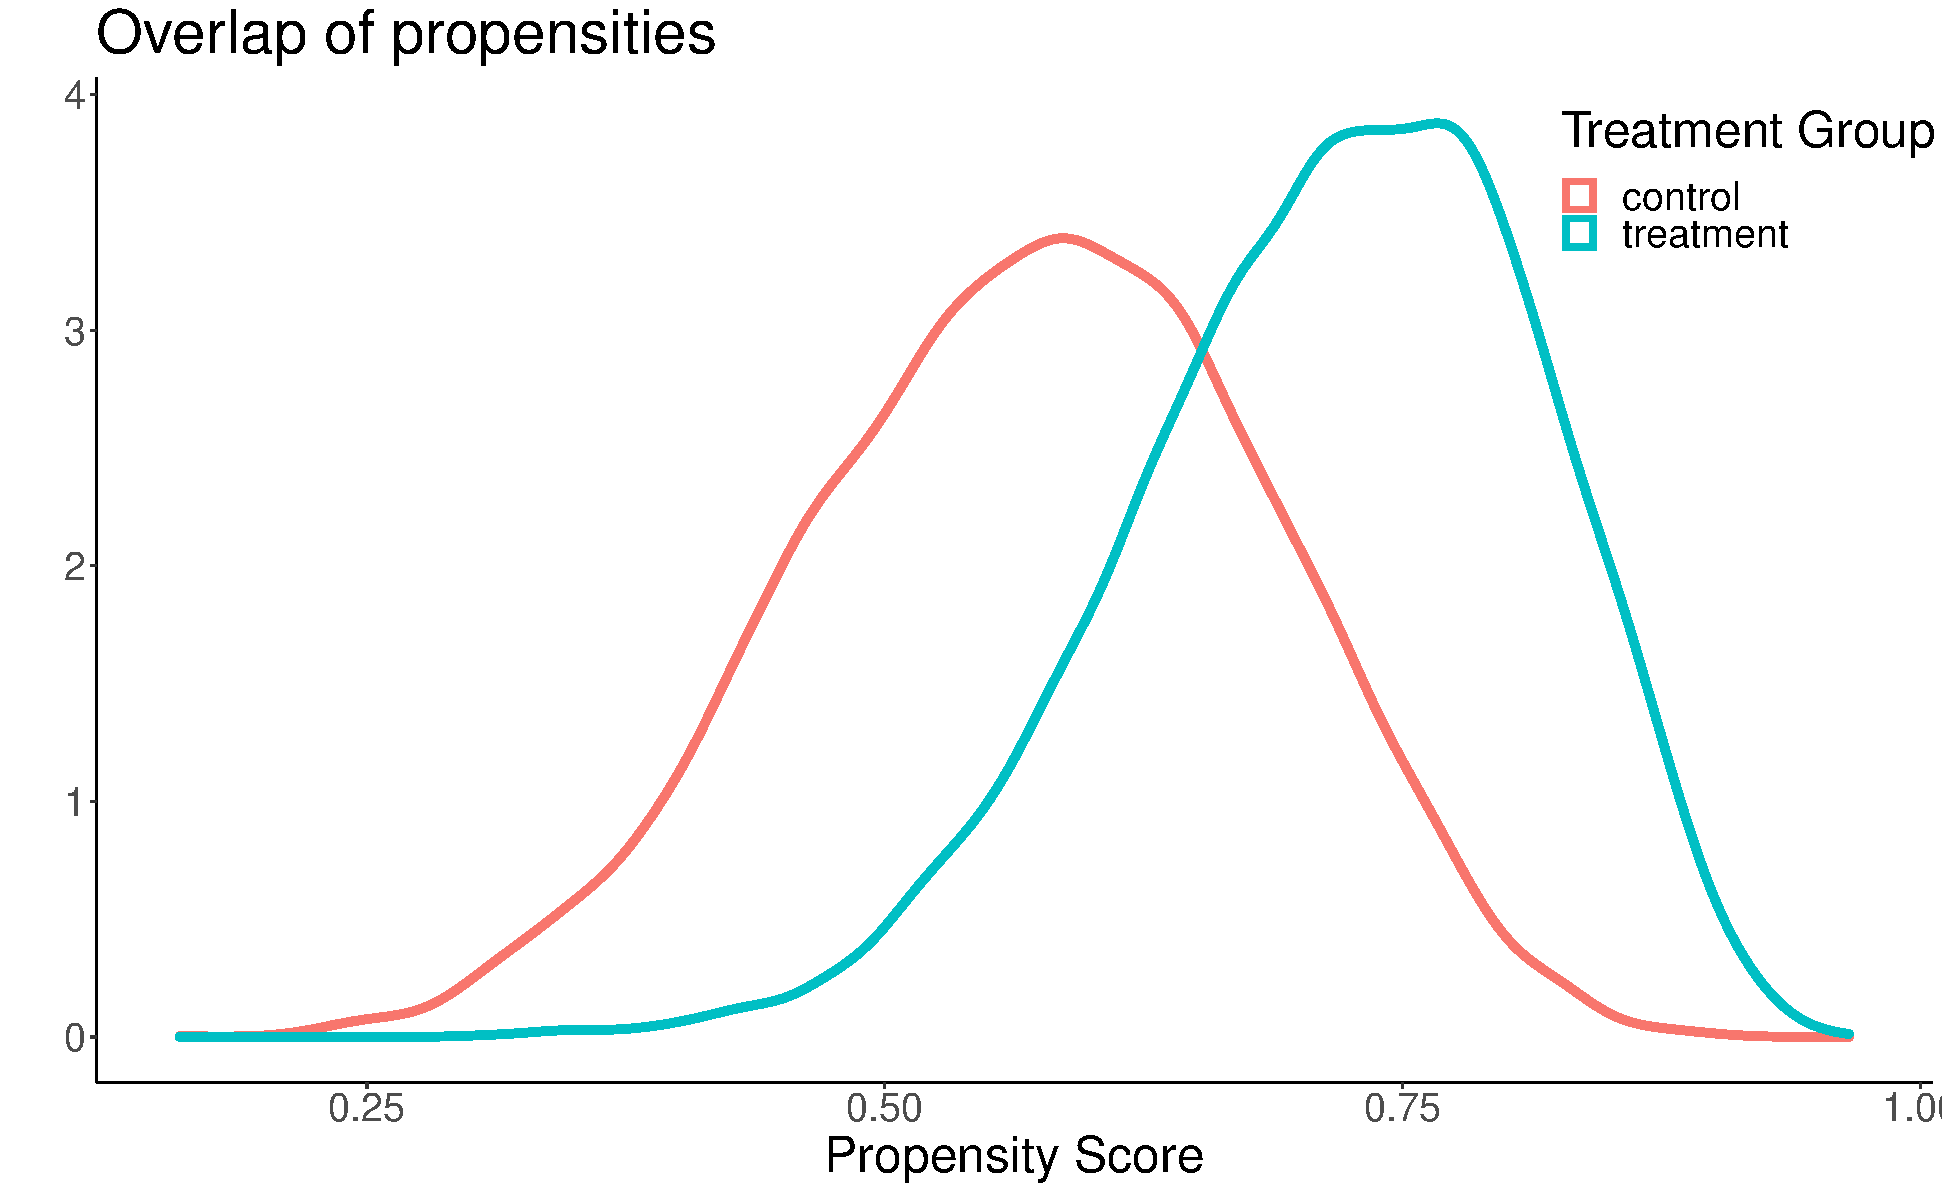
\includegraphics[width=\linewidth]{../lectures/images/overlap1.pdf}
\caption{Overlap in the propensity scores for example treated and control populations}
\end{figure*}        

As we go forward in thinking about random variation in $D_{i}$, it is convenient  to consider  the following economic model (from \citet{heckman1997instrumental}):
\begin{align*}
  Y_{i}(0) &= g(X_{i}, D_{i} = 0) + U_{i0}\\
  Y_{i}(1) &= g(X_{i}, D_{i} = 1) + U_{i1}\\
  Y_{i} &= g(X_{i},0) + D_{i}\left(\underbrace{g(X_{i},1) - g(X_{i},0)}_{\text{Average Population Gain}} + \underbrace{U_{i1} - U_{i0}}_{\text{idiosyncratic gain}}\right) + U_{i0}
\end{align*}
Now, we consider what drives the decision making for $D_{i}$:
\begin{equation*}
  D_{i} = 1( (Y_{i}(1) - Y_{i}(0))   + \kappa + V_{i}  > 0)
\end{equation*}
In other words, when the value is sufficiently high (above some overall + idiosyncratic cost $\kappa+V_{i}$), I choose to take the program. This creates obvious correlation between $D_{i}$ and $(Y_{i}(0), Y_{i}(1))$. 

WIth this setup, we can consider under what settings controlling for $\bX$ will be sufficient to recover a causal estimand. The easiest is when there are constant effects, e.g.  $U_{i1} - U_{i0} = 0$ for everyone. In this case, random variation in $V_{i}$ is what drives takeup, and is unrelated to the outcome. This makes life easy for us, but is not very interesting and also means there is no underlying heterogeneity in the treatment effect beyond what we observe in the characteristics. 

The other case is when the \emph{expected} gains to the program is the same for everyone ($E(U_{i1} - U_{i0}| X_{i}) = 0$), perhaps because of lack of information on the part of the individuals'. Then, while there may be ex post differences in treatment effects, they are not ex ante anticipated by the individuals and consequentially selected on.

The propensity score in this model is:
\begin{equation*}
  Pr(D_{i} = 1 | X_{i}) = Pr\left(g(X_{i},1) - g(X_{i},0) + \kappa + (U_{i1} - U_{i0}) > V_{i} \right) 
\end{equation*}
This gives us a framework to consider the economic returns to individuals to take a program, as in \Cref{fig:overlap2}. What would it take to switch them into the program? 
\begin{enumerate}
\item Lack of choice: not always available
\item Large incentive: expensive
\item High personal returns: selects into a particular type of person.
\end{enumerate}

\begin{figure*}
  \label{fig:overlap2}
  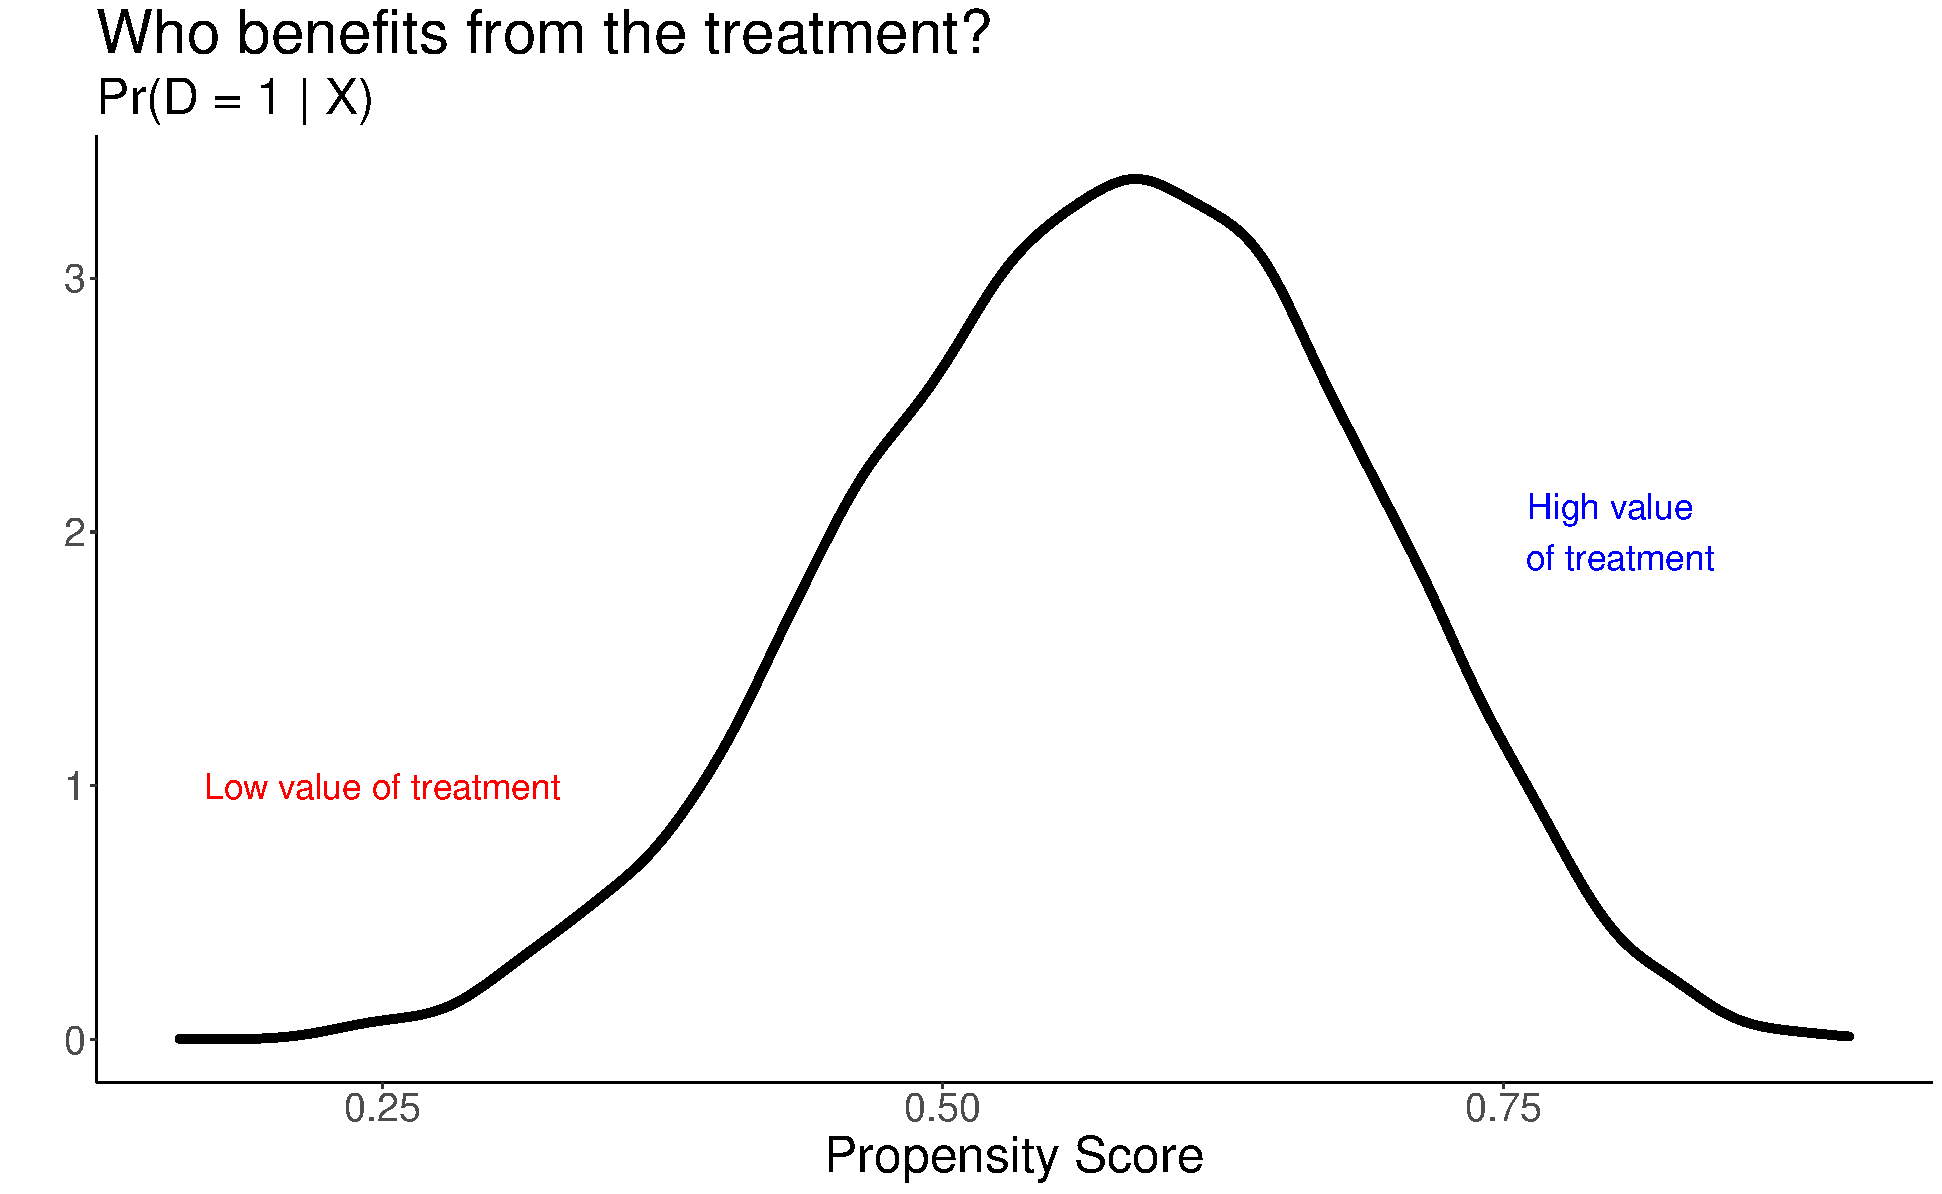
\includegraphics[width=\linewidth]{../lectures/images/overlap3.pdf}
  \end{figure*}

It is useful to remember this graph when considering how to induce participation. Some folks may just not want to participate. This could be perceptions on the returns (e.g. $Y(1) - Y(0)$), rightly or wrongly, but as a consequence, they  will be expensive to move. The estimand of interest will be considering parts of this distribution, and hence it si important to consider this when thinking about external validity.

Going forward, it is helpful to consider the propensity score as an index of valuation. We are hence looking for things that vary individuals' valuation and do not correlate with the potential outcome. In design-based work in economics, this is often referred to as an \emph{instrument}, and is a crucial part of the design-based research. 



\bibliography{lecture_note_bib.bib}
\bibliographystyle{plainnat}



\end{document}